\documentclass[12pt,a4paper]{article}


\usepackage[utf8]{inputenc}        % Кодировка UTF-8
\usepackage[T2A]{fontenc}          % Поддержка кириллицы
\usepackage[russian]{babel}        % Русский язык

\usepackage{graphicx}              % Вставка изображений
\usepackage{circuitikz}            % Рисование электрических схем
\usepackage{gensymb}

\title{Отчёт по выполнению КПЗ №2}
\author{Есиков С.Д, Иванова А. Я.}
\date{\today}

\begin{document}
	\maketitle
	
	\section*{Условия}
	Был выбран вариант № 16, который соответствует следующим параметрам контура
	\begin{itemize}
		\item Ёмкость катушки ($L$) -- 470 мкГн
		\item Сопротвление катушки ($R_L$) -- 4 Ом
		\item Частота резонанса контура ($f_o$)-- 32 кГц
	\end{itemize}
	\newpage
	
	\centering
	
	\section*{Таблица расчётов}
	
	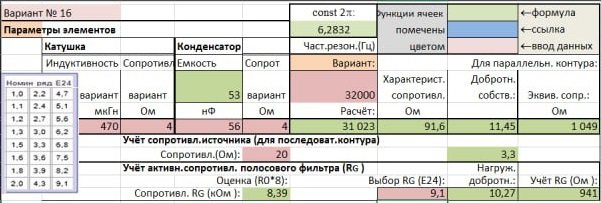
\includegraphics[width=0.7\linewidth]{src/calculate}

	\paragraph*{В результате для исходного фильтра:}
	\begin{enumerate}
		\item Ёмкость ($C$) -- $56 \: nF$
		\item Частота резонанса ($f_0$) -- $31.023 \: kHz$
		\item Хар. сопротивление ($\rho$) -- $91.6 \: Ohm$
		\item Добротность ($Q$) -- $11.45$
		\item Экв. сопротивление ($R_0$) -- $1.049 \: kOhm$
		\item Нагружающее сопротивление ($R_G$) -- $9.1 \: kOhm$
		\item Добротность с нагрузкой ($Q_G$) -- $10.27$
	\end{enumerate}

	\section*{Модель LC-фильтра}
	
	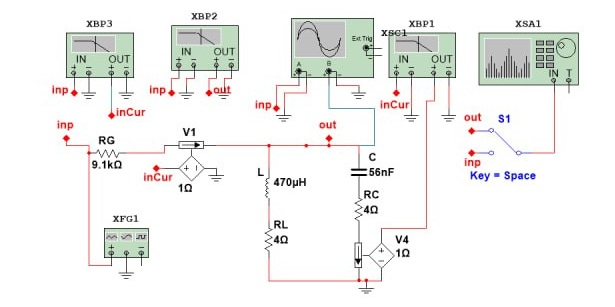
\includegraphics[width=\linewidth]{src/model_1}
	
	\section*{АЧХ и ФЧХ тока LC-фильтра}
	
	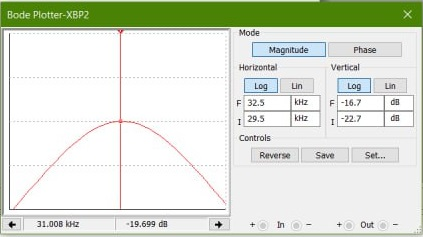
\includegraphics[width=0.4\linewidth]{src/MFH_1}
	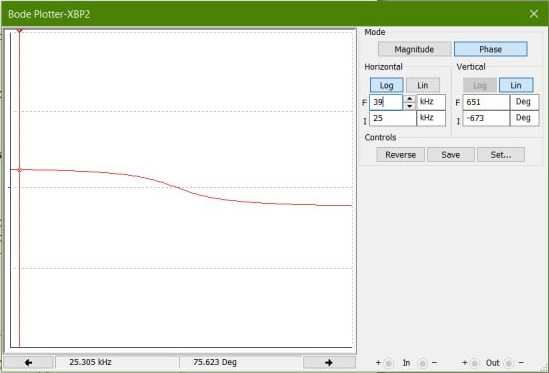
\includegraphics[width=0.4\linewidth]{src/FFH_1_1}
	
	\paragraph*{По графикам наблюдаем}
	\begin{itemize}
		\item Центральная частота: $31.008 \: kHz$ 
		\item Коэффициент передачи: $-19.699 \: dB$
		\item Полоса пропускания: $32.5 - 29.5 = 3 \: kHz$
		\item Добротность: $\frac{31.008}{3} = 10.336$
		\item Сдвиг фаз: $75.623 \: \degree$
	\end{itemize}
	
	\paragraph*{Различие с теоретическими расчётами пренибрежимо мало}
	
	\section*{Модель эквивалентного LC-фильтра}
	
	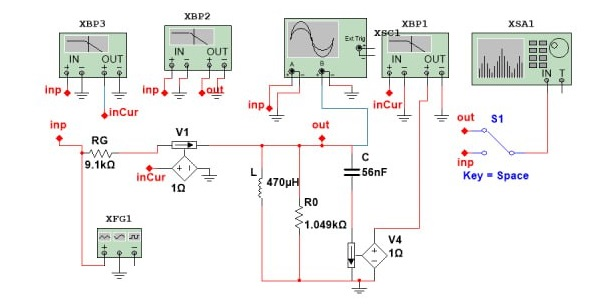
\includegraphics[width=\linewidth]{src/model_2}
	
	\section*{АЧХ тока эквивалентного LC-фильтра}
	
	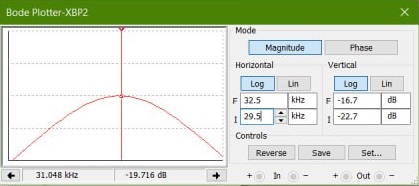
\includegraphics[width=0.5\linewidth]{src/MFH_2}
	
	\paragraph*{Новые значения}
	\begin{itemize}
		\item Центральная частота: $31.048 \: kHz$ 
		\item Коэффициент передачи: $-19.716 \: dB$
		\item Полоса пропускания: $3 \: kHz$
		\item Добротность: $\frac{31.048}{3} = 10.349$
	\end{itemize}
	
	\paragraph*{Результаты примерно сходятся с прошлыми, что подтверждает эквивалентность схем}
	
	\newpage
	
	\section*{Анализ фильтрации последовательных прямоугольных импульсов}
	
	\paragraph{Часота выбрана 5.84 kHz}
	
	\subsection*{Осцилограмма для 20\% скважности}
	
	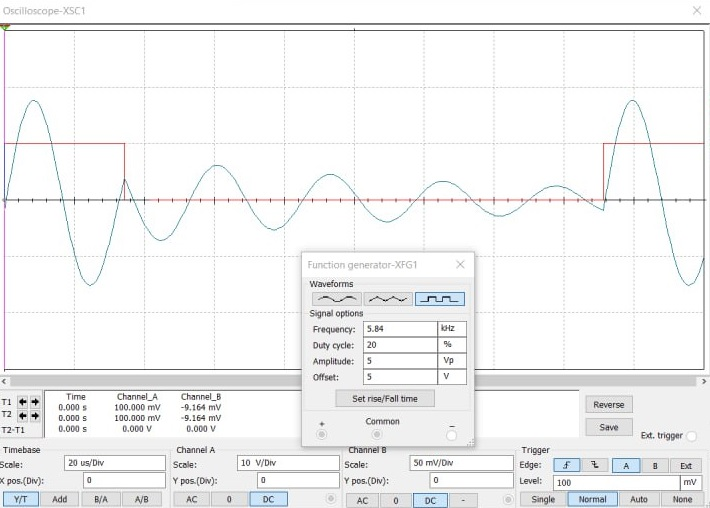
\includegraphics[width=0.7\linewidth]{src/oscil_2}
	
	
	\paragraph*{Видно, что из-за того, что обратный скачок сигнала происходит чуть позднее полного периода собственного колебания фильтра (что ожидаемо, учитывая что период скачка составляет примерно 1/5 * 5 периода колебания с учетом выбора частоты импульса как 1/5 частоты колебания), дальнейшие его колебания обладают почти нулевой запасённой энергией, что приводит к очень низкой амплитуде}
	
	\subsection*{Спектр}
	
	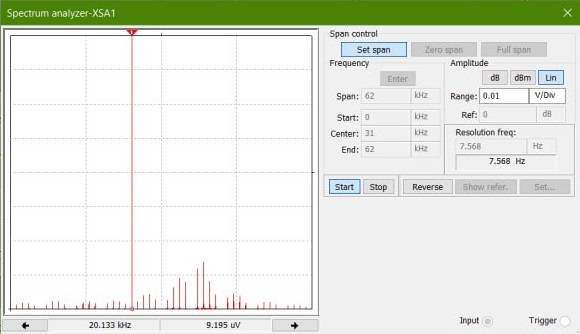
\includegraphics[width=0.7\linewidth]{src/spectr_2}
	
	\newpage
	
	\subsection*{Анализ фурье для 20\% скважности}
	
	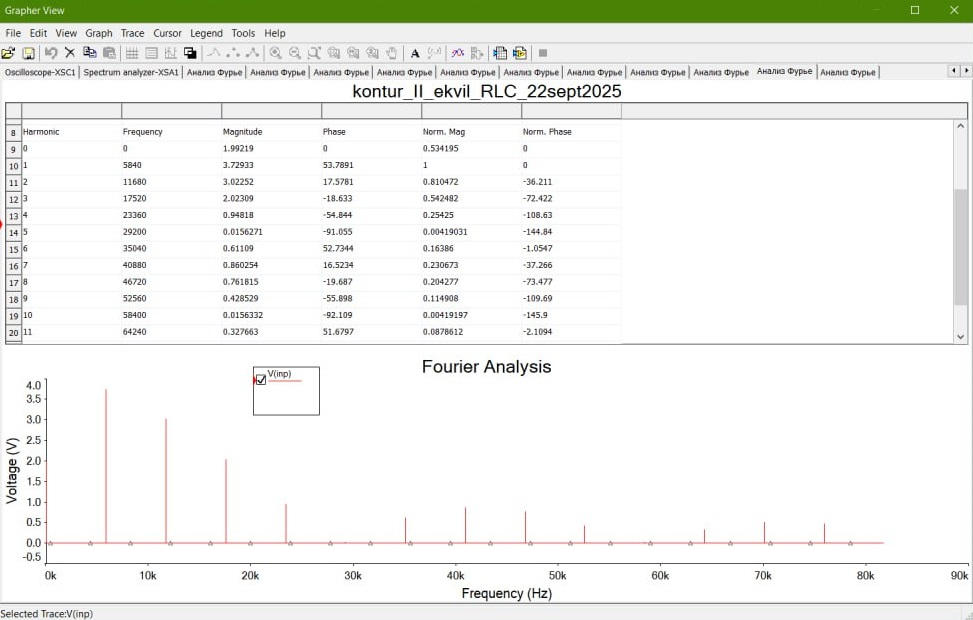
\includegraphics[width=0.7\linewidth]{src/fourier_in_20}
	
	\medskip
	\medskip
	\medskip
	\medskip
	\medskip
		
	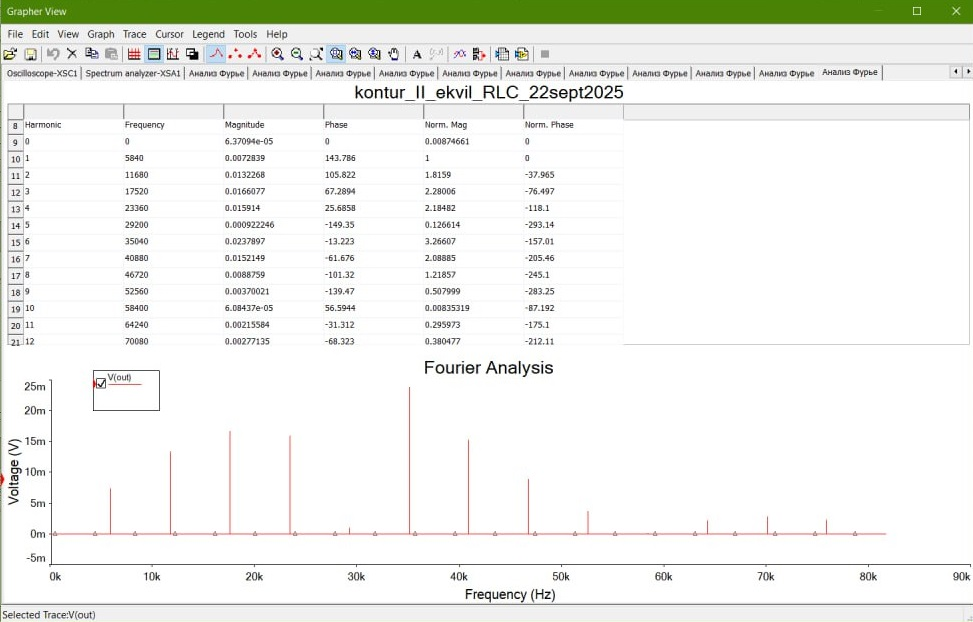
\includegraphics[width=0.7\linewidth]{src/fourier_out_20}

	\paragraph*{Отсутствие запасённой после скачка энергии не позволяет фильтру проявить свои свойства, потому результат анализа фурье выглядит как обычное почти нулевое колебание, где все гармоники вносят примерно один незначительный вклад}
	
	\subsection*{Осцилограмма для 10\% скважности}
	
	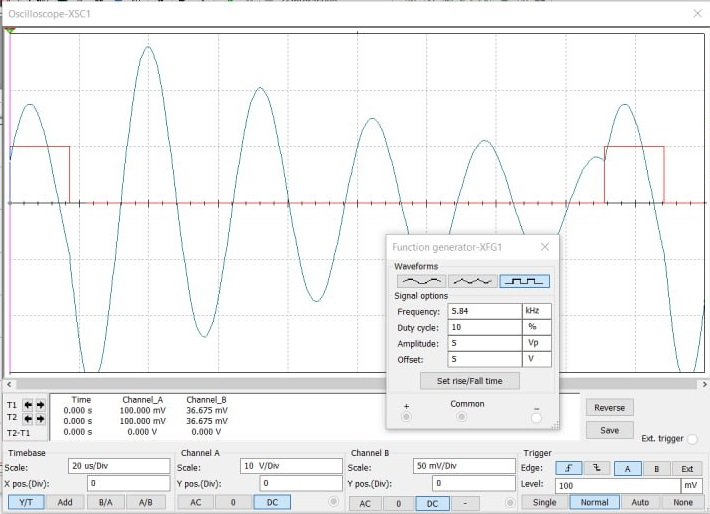
\includegraphics[width=0.7\linewidth]{src/oscil_1}
	
	
	\paragraph*{Здесь уже контур переходит в свободные колебания, с почти максимальной энергией внутри, что приводит к одной очень ярко выраженной гармонике, это также логично, ведь здесь уже период скачка составляет 1/10 * 5 = 1/2 периода колебания}
		
	\subsection*{Спектр}
	
	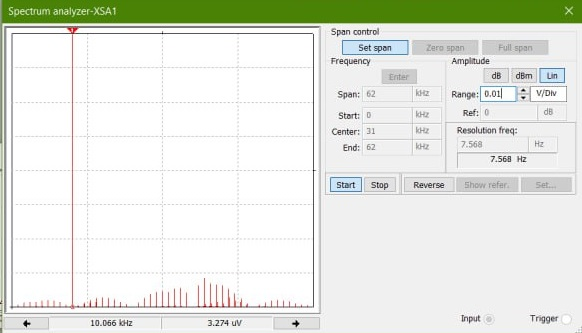
\includegraphics[width=0.7\linewidth]{src/spectr_1}
	
	\newpage
	
	\subsection*{Анализ фурье для 10\% скважности}
	
	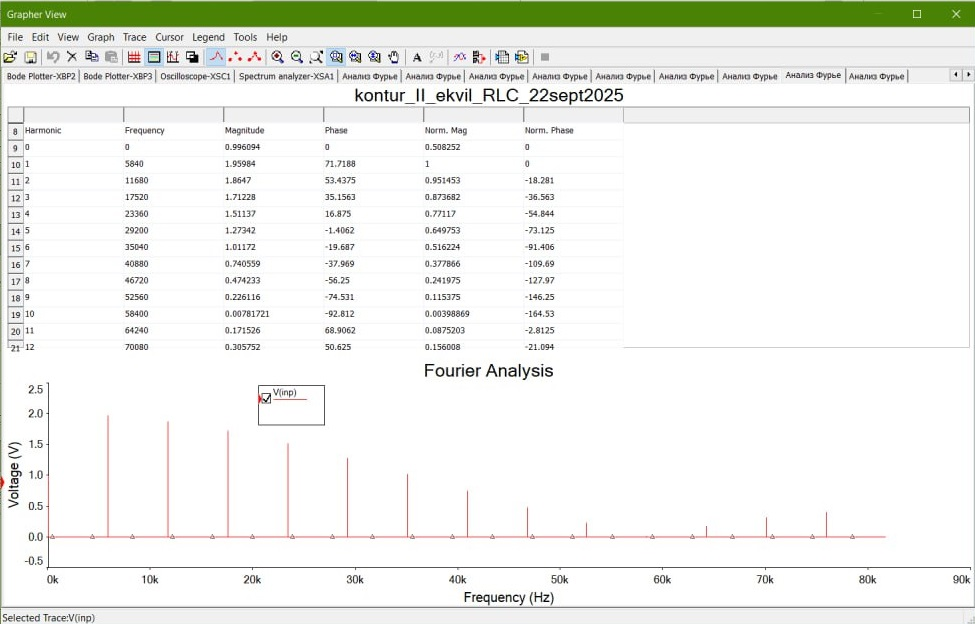
\includegraphics[width=0.7\linewidth]{src/fourier_in_10}
	
	\medskip
	\medskip
	\medskip
	\medskip
	\medskip
	
	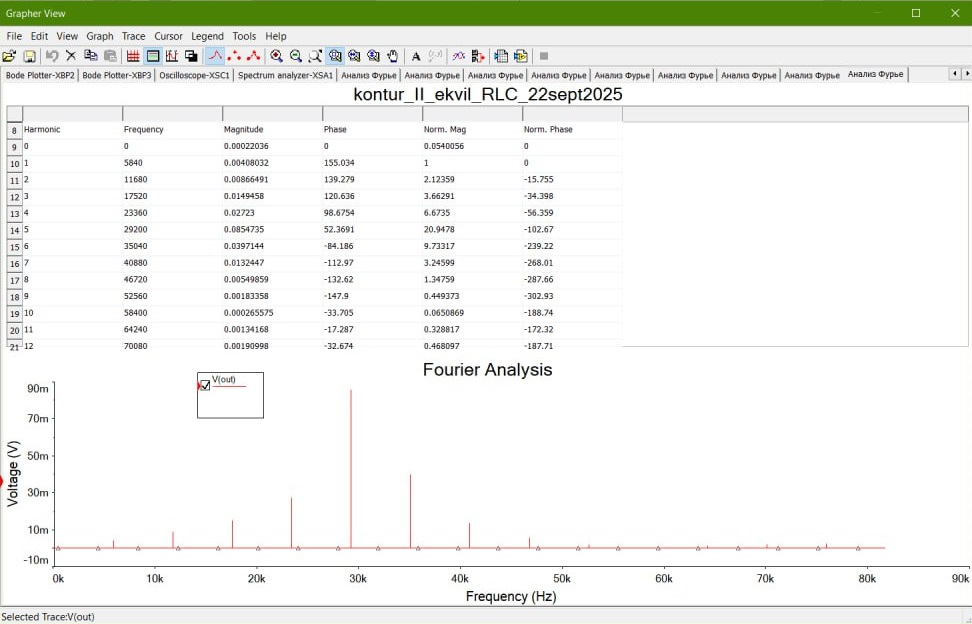
\includegraphics[width=0.7\linewidth]{src/fourier_out_10}
	
	
	\paragraph*{Тут видно насколько сильно больший вклад в форму выходного сигнала даёт гармоника на частоте близкой к центральной. Также заметно, что амплитуды остальнх гармоник почти не изменились при уменьшении скважности, но теперь из значения пренибрижимо малы по сравнению с главной гармоникой}
	
	\newpage
	
	\section*{Выводы}
	\begin{enumerate}
		\item Эксперементально полученные параметры фильтра сошлись с расчётным, что свидетельствует о корректности проведенных расчётов и построенной модели
		\item Вынос сопротивления реактивных элементов фильтра в отдельную паралельную нагрузку не привел к изменению параметров фильтра, что подтверждает эквивалетность схем
		\item Энергия запасаемая в контуре от прямоугольных импульсов зависит меньше от энергии самого импульса, сколько от сочетаемости скважности импульса и частоты колебаний контура (четность отношения периода скачка к полупериоды колебания)
		\item Полосовой LC-фильтр наглядно функционирует как частотный фильтр, чего и следовало ожидать
	\end{enumerate}
	
	
\end{document}